
\textbf{Observer le module de la transformée de Fourier. Quelle est la bande de fréquence utile pour le signal ?}
\begin{figure}[h]
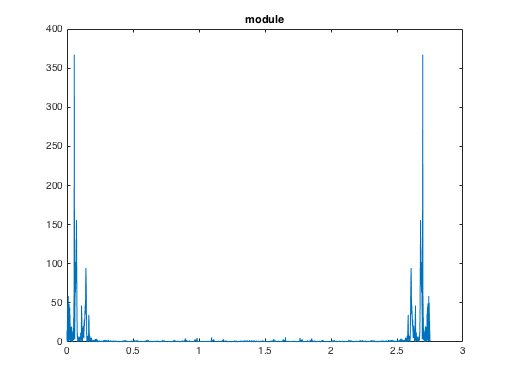
\includegraphics [width=.9\linewidth]{./img/module}
\caption{Module du signal issu de coucou.wav}
\end{figure}

La bande de fréquence utile pour le signal est [0 2.8]
\section{Filtre passe bas à réponse impulsionnelle finie}


\section{Filtre en peigne}

\section{Filtre passe Tout}

\section{Réverbération}